% !TeX program = xelatex
% !TeX encoding = UTF-8
% !TeX root = main.tex
\documentclass[UTF8,fontset=fandol,zihao=-4]{ctexart}
\usepackage{npu-report-style}
% 取消下一行注释以生成匿名送审版；保持注释则生成实名版。
% \npuanonymoustrue

% 基本信息与勾选项；开题次数和论文类型按本人确认填写。
\nputitle{非完备观测下动态世界模型的状态表征与预测研究}
\npuschool{电子信息学院}
\npuname{孙国栋}
\npunumber{2025100353}
\npumajor{信息与通信工程}
\npusupervisor{戴玉超}
\npudegree{博士}
\npudate{2026年10月08日}
\npucheckphdtrue
\npucheckfirsttrue
% \npuchecksecondtrue
\npucheckbasetrue
\npucheckapplytrue
% \npucheckenginetrue
% \npucheckoveralltrue

\hypersetup{pdftitle={\npuinnertitle}}
\ifnpuanonymous
  \hypersetup{pdfauthor={}}
\else
  \hypersetup{pdfauthor={\npuinnername}}
\fi

\begin{document}
\hypersetup{pageanchor=false}
\npuMakeCover
\npuMakeRequirements
\npuStartBody

\npuBlock*{学位论文研究依据}{学位论文的选题依据和研究意义，国内外研究现状和发展态势，主要参考文献，以及已有的工作积累和研究成果。}
{\noindent\kaishu （图、文、参考文献格式参照《西北工业大学博士研究生学位论文编写规则》）\par}
% !TeX root = ../main.tex
\subsection{选题依据及研究意义}

理解真实物理世界的动态变化，并预判行为可能产生的后果，是人工智能形成自主交互能力的重要基础。世界模型通过内部状态联系历史观测、当前环境和未来演化，为环境理解和行动选择提供可推演的场景依据。这一方向也受到基础研究布局的关注，国家自然科学基金委员会于2026年发布了“空间智能与世界模型”专项项目申请指南通告\cite{nsfcworldmodel2026}。如何从视觉观测中构建可靠的动态世界模型，是环境理解走向自主交互必须回答的问题。

真实物理世界持续演化，而视觉观测是离散、局部且不完整的。图~\ref{fig:dynamic-world-motivation} 借用 PhysTwin 的同一布料提拉案例素材\cite{phystwin2025}，概念性说明本课题拟研究的状态构建、随观测更新及动作条件演化过程，并不表示原论文已实现图中的全部能力。两帧历史观测只提供离散时刻和局部表面的信息，本课题拟由此构建可随新观测修正的三维状态，并在采样间隔内的 $\tau$ 处查询；给定动作 $\mathbf a$ 后，状态推演的未来与真实执行帧对照，后者仅用于评价。图中三维状态和预测画面取自原工作，连续时间轴、查询及更新箭头为本课题添加的概念标注。

% !TeX root = ../main.tex
% Background paradigm, not a method architecture or a four-task roadmap.
% Matrix: rows are representation levels (observation / 3D state),
% columns are time (t1 / t2=t / t+dt). Time runs left to right only.
% All photographs and model renders show the SAME PhysTwin cloth episode.
% State cutouts are pasted at one common cm/px scale, preserving the
% relative position of the two view-2 renders inside the 477x320 frame.
% Original JPEG panels, extraction map and SHA-256: materials/phystwin_cloth/.
% Axis, tau marker, arrows and labels are explanatory, not measured.
\begin{figure}[H]
  \centering
  \begingroup
  \definecolor{motInk}{HTML}{26343E}
  \definecolor{motMuted}{HTML}{6C7780}
  \definecolor{motLine}{HTML}{D8DDE1}
  \definecolor{motBlue}{HTML}{426A85}
  \definecolor{motAction}{HTML}{A66E38}
  \resizebox{\linewidth}{!}{%
  \begin{tikzpicture}[
    x=1cm,y=1cm,line cap=round,line join=round,text=motInk,
    font=\fontsize{9.5pt}{12pt}\selectfont,
    mothead/.style={font=\heiti\fontsize{10pt}{12pt}\selectfont},
    motnote/.style={font=\fontsize{8.5pt}{10.5pt}\selectfont,text=motMuted},
    rownote/.style={font=\fontsize{8pt}{9.6pt}\selectfont,text=motMuted},
    motarrow/.style={-{Latex[length=1.6mm,width=1.1mm]},draw=motBlue,line width=0.85pt},
    actarrow/.style={-{Latex[length=1.6mm,width=1.1mm]},draw=motAction,line width=0.9pt}
  ]
    \path[use as bounding box] (0,0) rectangle (15.6,7.10);

    % ---- time axis: it also serves as the column header ----
    \draw[motMuted!55,line width=0.5pt,-{Latex[length=1.3mm]}]
      (1.9,6.53) -- (15.15,6.53);
    \foreach \xx in {3.75,8.05,13.3}{%
      \draw[motMuted!70,line width=0.5pt] (\xx,6.53) -- (\xx,6.63);
    }
    \draw[motMuted!70,line width=0.5pt] (5.9,6.53) -- (5.9,6.63);
    \node at (3.75,6.78) {$t_1$};
    \node at (8.05,6.78) {$t_2=t$};
    \node at (13.3,6.78) {$t+\Delta t$};
    \node[motnote] at (5.9,6.78) {$\tau$};

    % ---- row labels: observation vs state ----
    \node[mothead] at (0.95,5.35) {视觉观测};
    \node[rownote] at (0.95,5.00) {离散、局部};
    \node[mothead] at (0.95,1.76) {三维状态};
    \node[rownote] at (0.95,1.41) {连续、可更新};

    % ---- observation row ----
    \node[anchor=north west,inner sep=0pt] at (1.9,6.383)
      {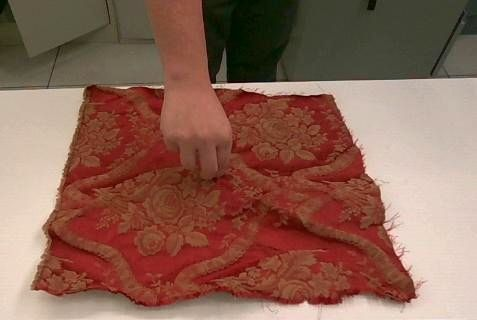
\includegraphics[width=3.7cm]{figures/materials/phystwin_cloth/observation_t1.jpg}};
    \draw[motLine,line width=0.35pt] (1.9,3.901) rectangle (5.6,6.383);
    \node[anchor=north west,inner sep=0pt] at (6.2,6.383)
      {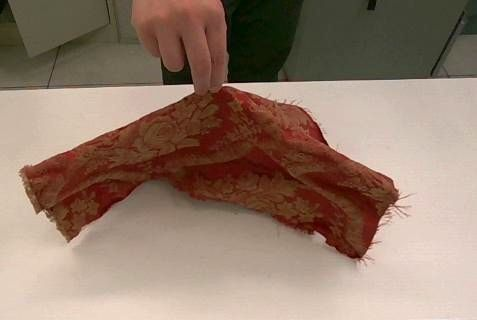
\includegraphics[width=3.7cm]{figures/materials/phystwin_cloth/observation_t2.jpg}};
    \draw[motLine,line width=0.35pt] (6.2,3.901) rectangle (9.9,6.383);
    \node[anchor=north west,inner sep=0pt] at (11.45,6.383)
      {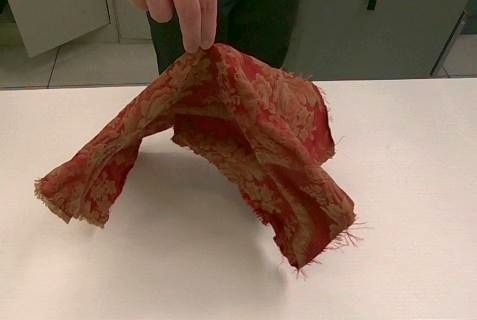
\includegraphics[width=3.7cm]{figures/materials/phystwin_cloth/execution_future.jpg}};
    \draw[dashed,motMuted!85,line width=0.55pt]
      (11.45,3.901) rectangle (15.15,6.383);

    % ---- state row: common scale k = 3.7cm / 280px ----
    % crop frame x=32..312, y=67..279 of the 477x320 renders
    \node[anchor=north west,inner sep=0pt] at (2.0057,2.5149)
      {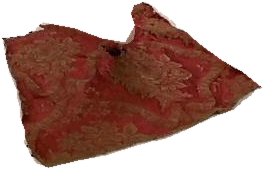
\includegraphics[width=3.4886cm]{figures/generated/world_model_paradigm/state_t1_view2_cutout.png}};
    \node[anchor=north west,inner sep=0pt] at (6.5832,2.8189)
      {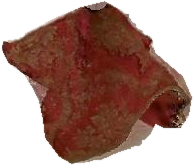
\includegraphics[width=2.5636cm]{figures/generated/world_model_paradigm/state_t2_view2_cutout.png}};
    \node[anchor=west,inner sep=0pt] at (11.45,1.5505)
      {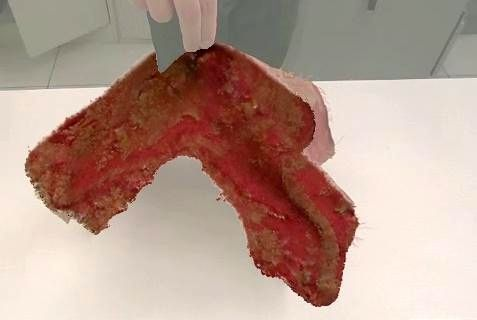
\includegraphics[width=3.7cm]{figures/materials/phystwin_cloth/prediction_future.jpg}};
    \draw[motLine,line width=0.35pt] (11.45,0.3095) rectangle (15.15,2.7915);
    % The prediction is a render of the same scene as the photographs; label it
    % explicitly so that it cannot be read as a captured frame.
    \node[anchor=south west,inner sep=2.2pt,fill=white,fill opacity=0.88,
      text opacity=1,font=\fontsize{8pt}{9.6pt}\selectfont]
      at (11.53,0.42) {模型预测};

    % ---- build / update the state from observations ----
    \draw[motarrow] (3.75,3.901) -- (3.75,2.951);
    \node[motnote,anchor=west] at (3.87,3.45) {构建};
    \draw[motarrow] (8.05,3.901) -- (8.05,2.951);
    \node[motnote,anchor=west] at (8.17,3.45) {更新};

    % ---- current state + given action -> forecast ----
    \draw[actarrow] (9.3,1.5505) -- (11.45,1.5505);
    \node[motnote,text=motAction] at (10.375,1.85) {给定动作 $\mathbf a$};

    % ---- the real future frame is a reference only, not an input ----
    \draw[dashed,motMuted,line width=0.6pt,
      {Latex[length=1.3mm]}-{Latex[length=1.3mm]}]
      (13.3,3.901) -- (13.3,2.7915);
    \node[motnote,anchor=west] at (13.42,3.45) {对照};

    % ---- tau: the state can be queried inside a sampling interval ----
    \draw[dashed,motMuted!55,line width=0.45pt] (5.9,6.53) -- (5.9,2.951);
    \fill[white] (5.9,2.951) circle (0.055);
    \draw[motMuted!55,line width=0.45pt] (5.9,2.951) circle (0.055);
    \node[motnote,anchor=west] at (6.02,3.19) {可查询};
  \end{tikzpicture}%
  }
  \endgroup
  \caption{连续动态世界模型的状态构建与演化预测概念示意（PhysTwin 案例素材）}
  \label{fig:dynamic-world-motivation}
\end{figure}


可靠状态的构建首先受到观测歧义及历史联系有效性的共同制约。有限图像只直接约束部分时刻和可见区域，快速运动、相机运动及遮挡相互叠加时，多种几何和运动解释可能同时符合观测。模型需要利用跨时刻运动联系组织证据，将逐渐显露的已有表面纳入所属对象或部件，使局部信息能够稳定累积；切割、撕裂等真实结构变化又可能使原有邻接和共享运动联系失效。若无差别地沿用历史，局部误差和失效约束可能传递到其他区域；若整体放弃历史，又会损失未变化部分的有效信息。因此，连续状态构建的关键在于，使运动表达、空间组织及局部更新同实际可获得的证据相适应。

面向交互预测，世界状态还需要为后续响应提供有效的初始条件。当前几何相近的场景，可能具有不同的运动方向、速度或连接关系，从而在相同动作下产生不同后果。对已观测场景的准确恢复，为预测提供了起点，但运动历史和有效结构能否转化为可靠的响应约束，仍需通过动作条件演化加以检验。观测区间内的重建可以利用区间中的多时刻信息，未来预测则应从当时已经获得的历史出发，推演给定动作下尚未发生的变化。由此，状态质量既体现为对已有场景的解释能力，也体现为对未来几何和运动变化的预测价值。

近年来，相关研究的快速发展为上述问题提供了方法基础。四维动态场景重建和学习式三维感知，丰富了从视频恢复几何、估计运动及累积场景信息的途径\cite{cndynamicgs2026,monst3r2025,cut3r2025}。世界模型通过状态演化学习，将环境预测引入行为学习及交互建模\cite{cnworld2026,ref02}；视觉语言动作模型等具身学习方法，则推动视觉语义知识向机器人操作迁移\cite{cnvla2026}。这些方向已在状态恢复、历史利用和动作响应上形成多种探索，其观测条件、表示形式及建模目标各有侧重，为进一步研究场景状态构建同交互预测之间的联系创造了条件。

基于上述认识，本课题围绕连续动态世界模型的构建方法开展研究，关注有限观测如何形成可连续查询、可随观测修正并能约束动作后果的三维动态状态。其科学意义在于，阐明观测证据、连续运动表达和有效结构约束对状态形成及演化预测的共同作用，认识可信历史的积累、局部调整和预测使用之间的联系。在应用层面，这类模型有望为动态目标的接触位置和动作时机判断、局部操作影响范围的推演提供场景依据。课题以代表性三维动态场景和选定具身操作为验证载体，形成可逐步衔接的构建方法及研究原型，检验状态构建的改进能够在何种条件下转化为预测和动作选择的收益。

\Needspace{110pt}
\subsection{国内外研究现状及发展态势}

连续动态世界模型的构建涉及从观测恢复场景状态、预测交互条件下的变化，以及利用预测支持行动。相关研究分别在四维动态场景重建、面向交互的世界模型和具身动作学习中形成多种路线，学习式三维感知也成为获取和更新场景状态的重要方法。以下沿这些领域的研究目标梳理进展，比较其状态形式、观测依据及演化条件，分析已有方法为本课题提供的基础和仍需研究的联系。

\Needspace{130pt}
\subsubsection{四维动态场景重建}

四维动态场景重建从图像或视频估计三维几何、外观及其随时间的变化，为动态世界状态提供场景基础。国内有关动态重建和神经辐射场的综述分别梳理了不同观测条件、表示方式及其应用\cite{cndynamic2024,cnnerf2025}。神经辐射场 NeRF 通过连续场函数联系图像和三维场景；D-NeRF、Nerfies 进一步引入时间条件或规范空间变形，使不同观测共享场景信息\cite{nerf2020,dnerf2021,nerfies2021}。HyperNeRF 采用高维表示描述拓扑变化的辐射场，扩展了规范空间映射可以处理的变化类型\cite{hypernerf2021}。神经场景流方法还联合表达随时间变化的场景和三维运动\cite{nsff2021}。这些隐式场由共享函数联系历史证据，变形及运动假设也约束了状态变化的表达。

显式图元表示则将几何和外观附着于可直接优化的场景元素。三维高斯泼溅为高效场景表达及可微渲染提供了基础\cite{gs2023}。Dynamic 3D Gaussians 保持图元属性，并以局部刚性约束运动；4D-GS 通过时空特征和变形模块驱动高斯；SC-GS 利用稀疏控制点共享运动\cite{dynamicgs2024,gs4d2024,scgs2024}。Deformable 3D Gaussians 从单目视频学习高斯变形，Gaussian-Flow 则采用时域与频域信息描述动态粒子的变化\cite{deformablegs2024,gaussianflow2024}。上述表示在图元延续方式和运动共享范围上的不同选择，影响着几何恢复和时间一致性。

运动约束进一步推动了场景的空间组织。MoSca 以稀疏运动支撑图驱动变形并融合观测，Shape of Motion 采用共享刚体运动基恢复持久三维轨迹，MovingParts 从粒子轨迹及部件运动中发现空间结构\cite{ref05,shapeofmotion2025,movingparts2024}。Consistent Instance Field 则在动态高斯中引入实例信息，区分可见性变化和持续身份\cite{consistentinstance2026}。运动支撑、运动分组和对象身份组织历史信息的层次不同，归属的可靠建立仍需结合几何、外观及可见性证据。

动态表面恢复关注几何联系如何随变化延续或调整。DynamicFusion 从深度观测联合恢复规范几何及非刚性运动，SobolevFusion 则利用隐式距离场演化处理自由非刚性变化\cite{dynamicfusion2015,sobolevfusion2018}。BundleSDF 在首帧对象掩码及刚体假设下联合进行 RGB-D 对象跟踪和神经表面重建\cite{bundlesdf2023}，其对象级位姿与可变形表面运动具有不同的建模条件。在显式表示中，GauSTAR 将高斯同网格绑定，在稳定区域延续联系、在变化区域解绑并重建；AT-GS 采用逐帧高斯面元优化和容量调整恢复表面；4DSurf 利用表面距离场流约束及重叠分段改善大形变下的几何和时间一致性\cite{gaustar2025,atgs2025,surf4d2026}。重建表示中的单元增减或连接调整，具有不同于物理材料边界新生的含义，后者需要由相应的几何和结构变化证据支持。

跨时刻对应是连接观测与运动的重要线索。RAFT 通过迭代更新估计两帧间的二维光流，RAFT-3D 则在 RGB-D 条件下利用刚体运动嵌入估计三维场景流\cite{raft2020,raft3d2021}。二维对应能够约束投影运动，但深度、相机位姿和可见性仍会影响其转化为三维运动的可靠性。

长时点跟踪进一步关注遮挡后的对应延续。TAPIR 结合逐帧匹配与时间精化，CoTracker 联合估计多个点的轨迹，CoTracker3 则利用伪标签扩展真实视频中的跟踪学习\cite{tapir2023,cotracker2024,cotracker3}。OmniMotion 使用整个视频进行优化并建立规范表示，以恢复长时二维轨迹\cite{omnimotion2023}。这些轨迹为跨时刻关联提供线索，但不同方法所允许的时间范围和遮挡处理方式不同，需要同连续状态恢复及在线使用的观测条件分开比较。

学习式三维感知为场景恢复引入了跨场景先验，使状态获取逐渐从逐场景优化扩展到前馈推断及持续更新。MonST3R 直接估计动态场景的逐时刻三维点图，再结合后续对齐恢复整体几何及相机信息；CUT3R 通过随新观测更新的循环状态，在共同坐标系中读取三维点图\cite{monst3r2025,cut3r2025}。持续接收图像并更新内部状态，描述的是信息维护过程；在非采样时刻查询运动，则依赖相应的时间表达，两种能力需要分别认识。

图~\ref{fig:literature-reconstruction} 概括了动态场景恢复的几类可读取结果：上半部的 Shape of Motion 从同一视频观测恢复三维轨迹并以新视角呈现场景，下半部的 RetimeGS 则恢复两个采样时刻之间的中间状态\cite{shapeofmotion2025,retimegs2026}。跨时刻的运动联系、跨视角的空间内容和帧间状态由此形成直观参照，下面进一步考察时间表达及观测约束如何支持这些能力。

\begin{figure}[htbp]
\centering
\resizebox{\linewidth}{!}{% !TeX root = ../main.tex
% Section 1.2.1: authentic author outputs, not a shared-method benchmark.
% Panels and exact crops are recorded in materials/literature_review/.
% Natural subfigure layout: a lettered caption above each row and images set at
% a common height, with no panel frame. Frames are reserved for structure, not
% for grouping pictures that are already aligned.
\begingroup
\linespread{1}\selectfont
\begin{tikzpicture}[
  x=1cm,y=1cm,text=black,line cap=round,line join=round,
  font=\songti\fontsize{10pt}{12pt}\selectfont,
  every node/.style={align=center,outer sep=0pt,inner sep=0pt},
  lrTitle/.style={font=\heiti\fontsize{10.2pt}{12.5pt}\selectfont},
  lrNote/.style={font=\fontsize{9.2pt}{11.5pt}\selectfont},
  lrArrow/.style={draw=black,line width=0.65pt,
    -{Latex[length=1.7mm,width=1.15mm]}}
]
  \path[use as bounding box] (0,-0.05) rectangle (16,10.35);

  % ---- (a) Shape of Motion: observation, persistent tracks, novel view ----
  \node[lrNote] at (2.725,9.60) {输入观测};
  \node[lrNote] at (8.000,9.60) {三维轨迹};
  \node[lrNote] at (13.275,9.60) {新视角重建};
  \node[anchor=north west] at (0.35,9.32)
    {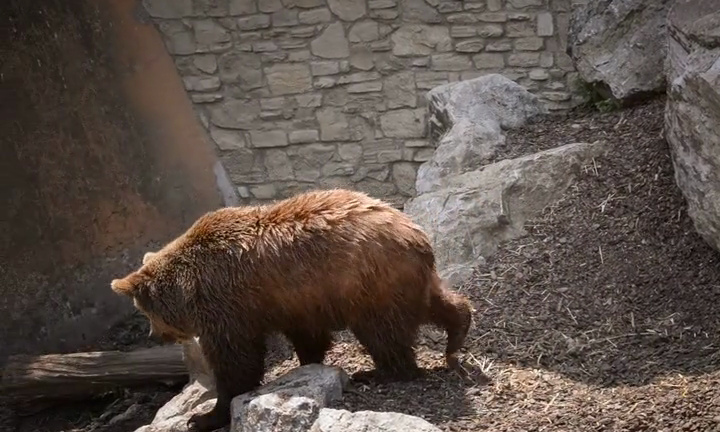
\includegraphics[width=4.75cm]{figures/generated/literature_review/som_observation.jpg}};
  \node[anchor=north west] at (5.625,9.32)
    {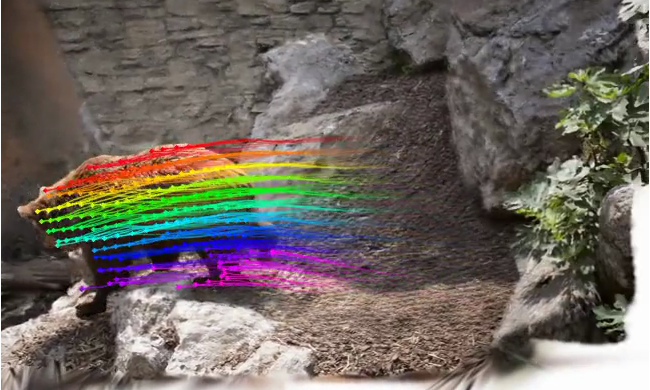
\includegraphics[width=4.75cm]{figures/generated/literature_review/som_tracks.jpg}};
  \node[anchor=north west] at (10.90,9.32)
    {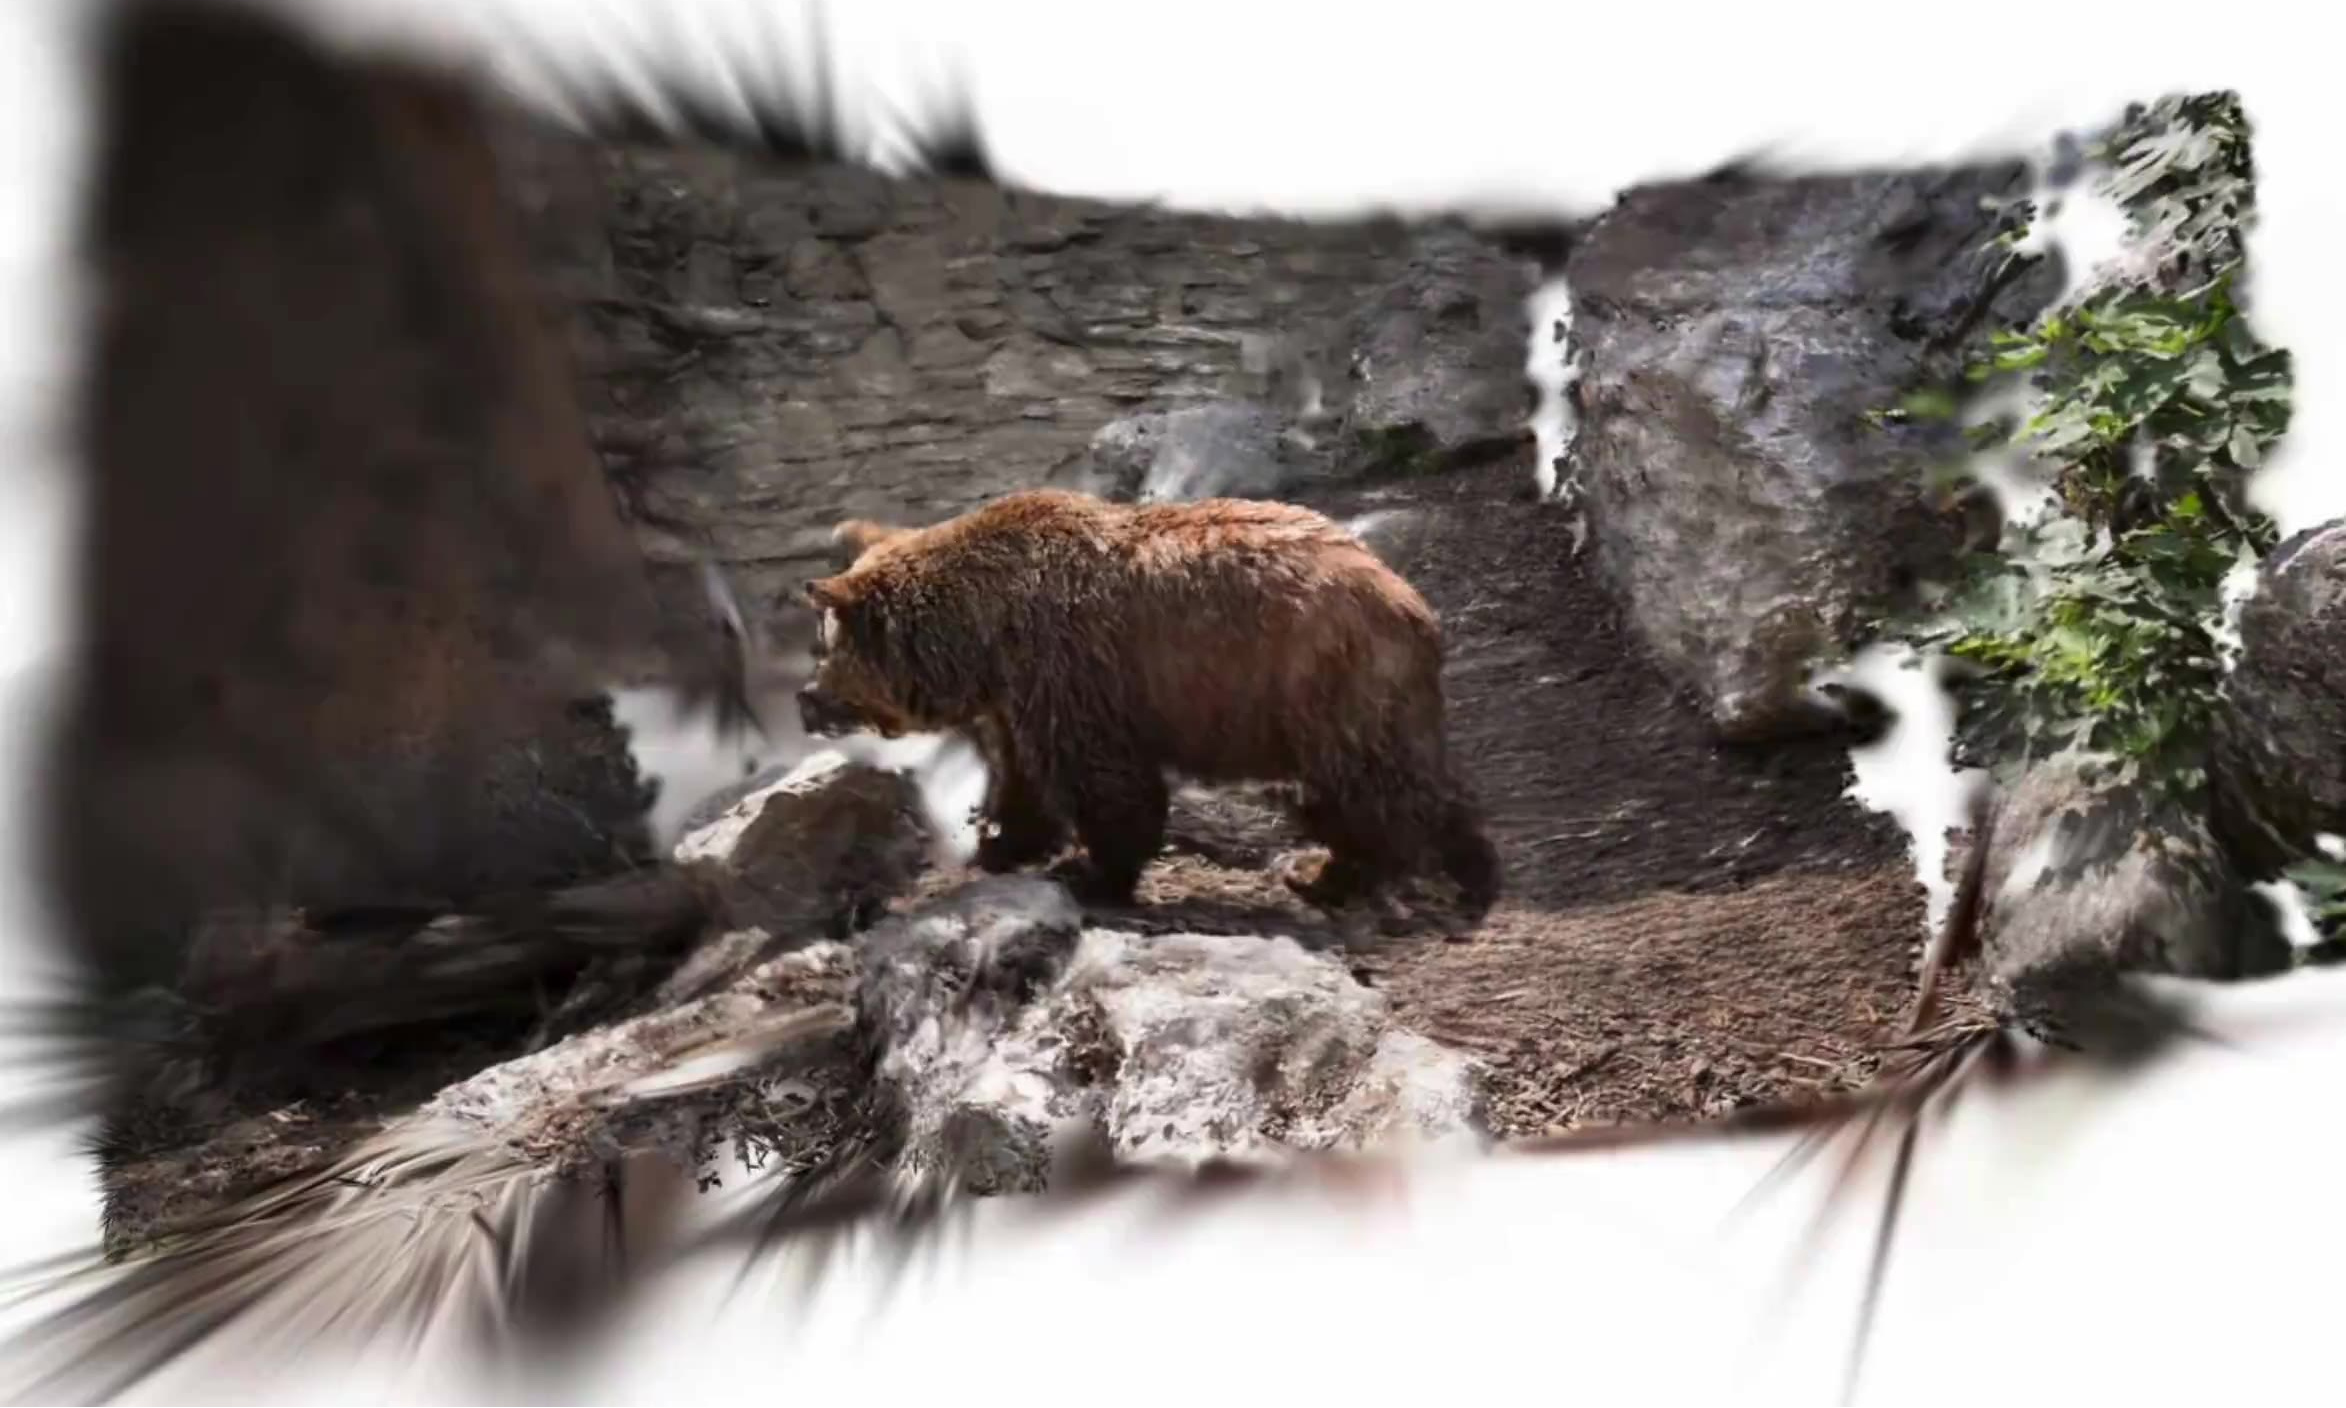
\includegraphics[width=4.75cm]{figures/generated/literature_review/som_novel_view.jpg}};
  \node[text width=7.6cm,align=center] at (8.000,6.00)
    {{\captionsetup[subfigure]{font=figsublittitle,skip=0pt}
      \subcaption{Shape of Motion}\label{subfig:lit-recon-som}}};

  \draw[black!25,line width=0.45pt] (0.10,5.66) -- (15.90,5.66);

  % ---- (b) RetimeGS: the same interval, with a non-sampled midpoint ----
  \node[lrNote] at (2.725,4.97) {采样时刻 $t_0$};
  \node[lrNote] at (8.000,4.97) {帧间时刻 $t_m$};
  \node[lrNote] at (13.275,4.97) {采样时刻 $t_1$};
  \node[anchor=north west] at (0.35,4.69)
    {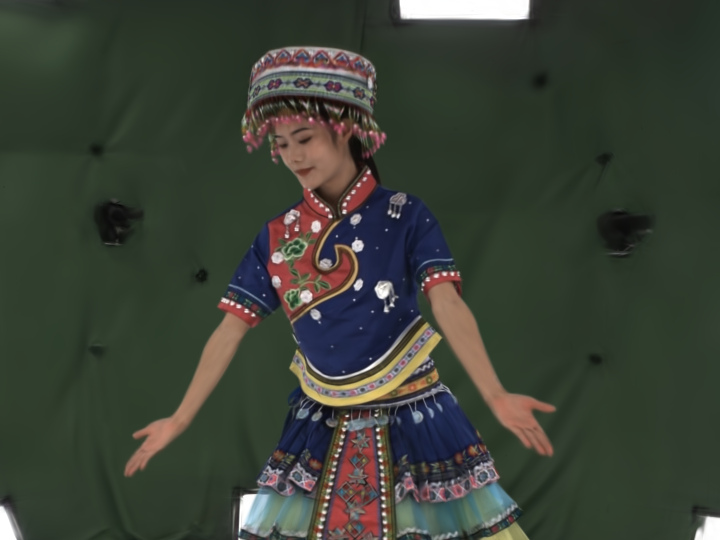
\includegraphics[width=4.75cm]{figures/generated/literature_review/retime_t0.jpg}};
  \node[anchor=north west] at (5.625,4.69)
    {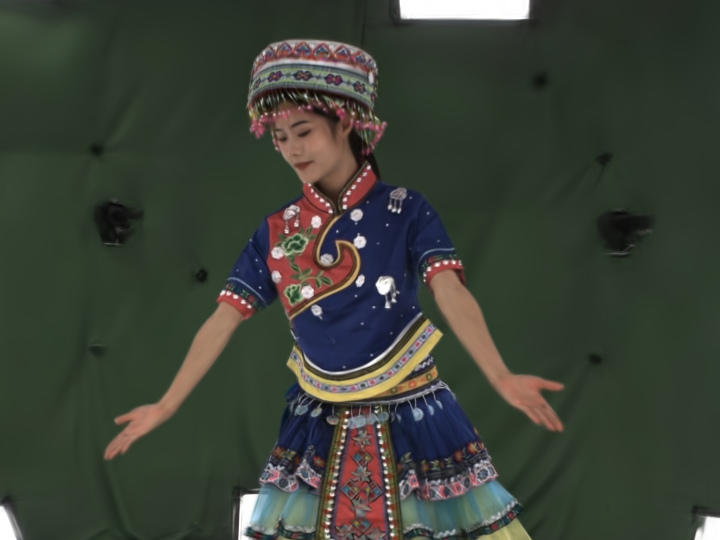
\includegraphics[width=4.75cm]{figures/generated/literature_review/retime_mid.jpg}};
  \node[anchor=north west] at (10.90,4.69)
    {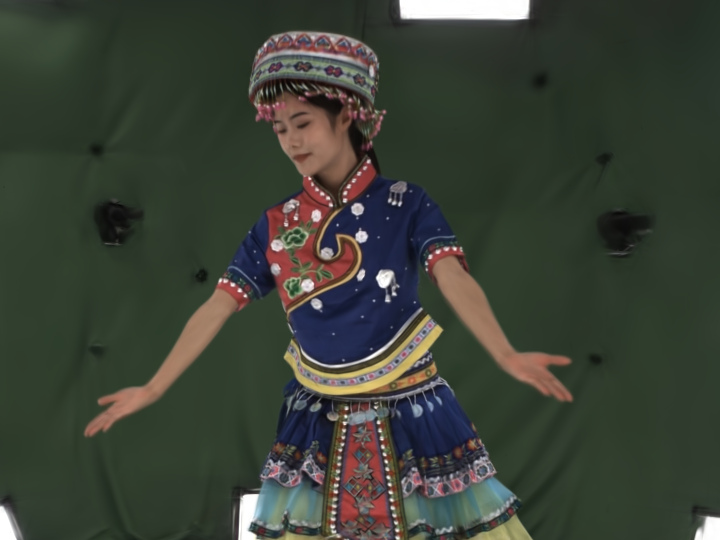
\includegraphics[width=4.75cm]{figures/generated/literature_review/retime_t1.jpg}};

  % The interval bar under the second row: sampled endpoints and the query time.
  \draw[lrArrow] (2.725,1.02) -- (13.45,1.02);
  \fill[black] (2.725,1.02) circle[radius=0.045];
  \draw[draw=black,fill=white,line width=0.7pt] (8,1.02) circle[radius=0.055];
  \fill[black] (13.275,1.02) circle[radius=0.045];
  \node[lrNote] at (8,0.72) {区间内任意时刻可查询};
  \node[text width=7.6cm,align=center] at (8.000,0.22)
    {{\captionsetup[subfigure]{font=figsublittitle,skip=0pt}
      \subcaption{RetimeGS：观测区间内插值}\label{subfig:lit-recon-retimegs}}};
\end{tikzpicture}
\endgroup
}
\caption{动态场景重建的代表性结果}
\label{fig:literature-reconstruction}
\end{figure}

在时间维度上，连续查询和未来外推已形成更具体的研究目标。RetimeGS 针对图中所示的帧间恢复问题，显式描述高斯的时间行为并加强插值监督，以减轻训练时刻之间的时间混叠；在采样过疏或帧间位移过大时，其插值仍受到对应可靠性的限制\cite{retimegs2026}。Zhang 等通过 SE(3) B 样条联合描述位置和朝向，利用自适应控制机制调整运动基及控制点数量，以兼顾运动表达能力和计算效率\cite{se3bspline2026}。ParticleGS 则通过连续动力学描述观测范围之外的运动\cite{particlegs2026}。这些方法分别侧重帧间恢复、轨迹表达及未来外推，所需观测和演化假设存在差异：区间内插值可以利用查询时刻两侧的观测，区间外外推则依赖已有历史。连续时间表达应同其监督条件和使用范围一并考察。

观测可靠性也开始直接参与这类动态状态的优化。USplat4D 估计随时间变化的高斯不确定性，利用时空图将可靠区域的运动信息传递到观测较弱的区域，改善遮挡条件下的几何和新视角合成\cite{usplat4d2026}。其研究表明，可靠证据的传播已经是动态重建的重要方向。结合连续轨迹和自适应运动表达的进展，还需进一步考察观测支持的时间范围、运动复杂程度及表达自由度如何共同影响恢复结果，以及这些影响能否通过非采样时刻的几何和运动质量得到验证。

可靠性估计还需要检查给出的置信程度是否同实际误差相符。深度集成和神经网络校准研究分别提供了预测不确定性与置信度评价的参考\cite{ensembles2017,calibration2017}；其中分类置信度的校准条件不能直接等同于连续三维运动的误差评价，具体应用仍需结合轨迹和几何参考检验。

对动态状态的评价也逐渐覆盖外观之外的几何及运动质量。DyCheck 分析真实采集条件下的动态重建和对应精度，TAP-Vid 与 TAPVid-3D 分别提供二维和三维轨迹及可见性评价依据\cite{dycheck2022,tapvid2022,tapvid3d2024}。总体而言，已有研究已从多种表示和求解方式建立时间联系、空间结构及表面更新机制。对于观测不完整且变化复杂的场景，仍需认识这些机制如何决定可信信息的共享范围，以及观测约束能在何种条件下支持稳定的连续状态。

\Needspace{130pt}
\subsubsection{面向交互的世界模型}

世界模型通过场景状态及其转移描述环境可能如何变化，其状态可以采用潜在变量、视觉特征或显式三维结构等形式。动作条件模型以给定行为推演后果，任务条件模型则依据目标描述生成可能的未来。状态恢复和演化关系可以联合学习，也可以通过重建或物理建模衔接；所选择的状态需要保留对后续响应有用的信息，模型能力因而同输入条件和预测对象密切相关。

部分可观测条件下，单次观测通常不足以确定环境状态，相关决策理论通过历史信息和状态信念描述这一限制\cite{pomdp1998}。循环世界模型将压缩观测与潜在状态演化用于策略学习，MuZero 则围绕奖励、价值及策略预测学习支持规划的模型\cite{worldmodels2018,muzero2020}。两者都利用预测辅助决策，但内部状态不必直接对应度量三维几何。

潜在状态方法通过压缩视觉信息建立适于预测及控制的动力学。PlaNet 从图像学习潜在动力学，并利用模型规划动作；Dreamer 及 DreamerV3 以学习到的环境模型生成想象轨迹，进而改进行为\cite{ref01,dreamer2020,ref02}。I-JEPA 研究图像区域特征的预测，DINO-WM 则在预训练视觉特征空间预测动作条件变化，再优化动作序列以到达目标观测\cite{ijepa2023,ref03}。任务相关状态学习和预训练特征分别为预测提供依据，所得表示保留的信息由学习目标及数据共同决定。

在模型辅助控制中，PETS 使用概率动力学模型及集成估计支持动作规划，TD-MPC2 在学习到的潜在空间中优化候选轨迹\cite{pets2018,tdmpc2_2024}。模型预测用于选择动作时，其误差、不确定性和优化时域会共同影响控制效果，因此需要区分预测模型本身和基于预测的决策流程。

显式结构和物理约束为响应建模提供了另一类依据。图网络模拟器利用粒子间关系组织消息传递和演化，使局部结构参与动力学预测\cite{gns2020}。PhysTwin 从稀疏 RGB-D 交互视频重建可变形对象，以质点弹簧模型、几何及高斯外观构建可模拟的数字孪生，并在给定控制点运动下进行未来预测和新交互模拟\cite{phystwin2025}。这类方法将几何和物理约束直接用于演化，所得响应也依赖于所选物理模型及由观测识别的参数。

对象中心表示从另一角度组织场景信息。SAVi 在给定对象提示及运动监督的条件下从视频学习对象槽，SlotFormer 在对象槽表示上建模后续视觉动态\cite{savi2022,slotformer2023}。对象槽能够提供分解场景和组织交互的方式，但其潜在表示本身不等同于已标定的三维几何或材料连接。

生成式方法进一步将未来视频和三维场景作为预测对象。TesserAct 根据初始图像及任务指令联合生成 RGB、深度和法向视频，再将其转化为四维场景；GWM 根据历史状态和动作，在高斯潜在空间中生成未来场景\cite{tesseract2025,gwm2025}。任务条件的多模态几何生成和动作条件的高斯状态转移，提供了不同的未来场景接口，也将演化准确性和跨视角一致性纳入预测评价。

对空间记忆和三维局部响应的研究则进一步丰富了状态形式。PERSIST 以持续的潜在三维场景组织环境、相机及渲染过程，改善长时间生成中的空间记忆和几何一致性\cite{ref10}。PointWorld 将场景状态和机器人动作统一到三维点及点流表示中，预测给定动作下的场景点位移\cite{ref06}，其局部响应的输入输出形式如图~\ref{fig:literature-prediction} 所示。

\begin{figure}[htbp]
\centering
\resizebox{\linewidth}{!}{% !TeX root = ../main.tex
% PointWorld, Fig. 16, physical PDF page 33, the first DROID cloth case.
% Both future panels refer to the same 1.0 s horizon and author rendering view.
% Reference annotations are distinct from model predictions; no execution is relabeled.
\begingroup
\linespread{1}\selectfont
\begin{tikzpicture}[
  x=1cm,y=1cm,text=black,line cap=round,line join=round,
  font=\songti\fontsize{10pt}{12pt}\selectfont,
  every node/.style={align=center,outer sep=0pt,inner sep=0pt},
  lpTitle/.style={font=\heiti\fontsize{10.5pt}{13pt}\selectfont},
  lpFrame/.style={draw=black,line width=0.65pt},
  lpPhoto/.style={anchor=north west},
  lpArrow/.style={draw=black,line width=0.8pt,
    -{Latex[length=1.8mm,width=1.2mm]}}
]
  \path[use as bounding box] (0,0) rectangle (16,6.65);
  \foreach \xl/\xr/\xc/\heading in {
    0.10/4.80/2.450/RGB观测（两视角）,
    5.40/10.35/7.875/模型预测,
    10.95/15.90/13.425/参考标注}{%
    \draw[lpFrame] (\xl,0.15) rectangle (\xr,6.50);
    \path[fill=black!5] (\xl+0.01,5.96) rectangle (\xr-0.01,6.49);
    \draw[lpFrame] (\xl,5.96) -- (\xr,5.96);
    \node[lpTitle] at (\xc,6.23) {\heading};
  }

  % RGB examples from the RGB-D inputs, with the given robot point-flow action.
  \node[lpPhoto] at (0.55,5.70)
    {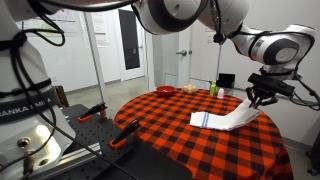
\includegraphics[width=3.80cm]{figures/generated/literature_review/point_observation_v1.jpg}};
  \node[lpPhoto] at (0.55,3.42)
    {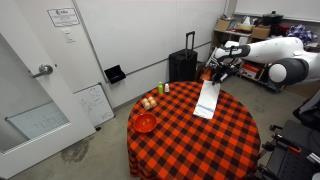
\includegraphics[width=3.80cm]{figures/generated/literature_review/point_observation_v2.jpg}};
  \draw[draw=black!55,line width=0.4pt] (0.55,3.5625) rectangle (4.35,5.70);
  \draw[draw=black!55,line width=0.4pt] (0.55,1.2825) rectangle (4.35,3.42);
  \draw[lpFrame] (0.35,0.35) rectangle (4.55,0.98);
  \node at (2.45,0.665) {给定机器人点流 $a_{0:T}$};
  \draw[lpArrow] (4.86,3.10) -- (5.34,3.10);

  \node[lpPhoto] at (5.55,5.55)
    {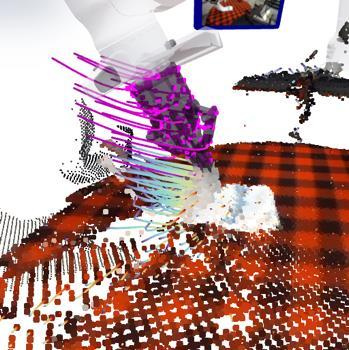
\includegraphics[width=4.65cm]{figures/generated/literature_review/point_prediction_1s.jpg}};
  \node[lpPhoto] at (11.10,5.55)
    {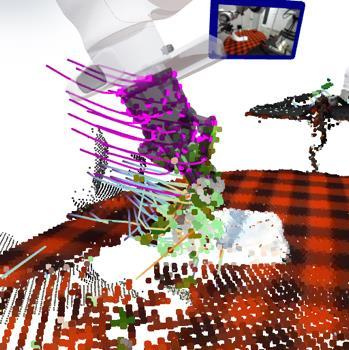
\includegraphics[width=4.65cm]{figures/generated/literature_review/point_reference_1s.jpg}};
  \draw[draw=black!55,line width=0.4pt] (5.55,0.90) rectangle (10.20,5.55);
  \draw[draw=black!55,line width=0.4pt] (11.10,0.90) rectangle (15.75,5.55);
  \node at (7.875,0.53) {$t_0+1.0\,\mathrm{s}$};
  \node at (13.425,0.53) {$t_0+1.0\,\mathrm{s}$};
\end{tikzpicture}
\endgroup
}
\caption{动作条件下的三维场景预测}
\label{fig:literature-prediction}
\end{figure}

图中的同一布料案例将这种预测具体呈现为三维点流：模型根据 RGB-D 观测和给定机器人点流预测场景点运动，左侧呈现输入中的两视角 RGB，中央预测和右侧参考标注则对应相同的 $1\,\mathrm{s}$ 未来时域\cite{ref06}。局部操作的影响因而可以通过三维点流观察，而预测所需的初始运动信息还取决于模型实际接收的历史范围。

围绕空间记忆及未来三维状态，FR3D 在预训练重建表示的潜在空间中预测动态场景，并区分自运动的影响；Flow Equivariant World Models 则以运动等变的潜在记忆维护部分观测下的环境信息\cite{ref07,ref08}。多视角掩蔽世界模型研究利用多个相机视图学习操作表征\cite{mvmwm2023}，但空间视角的缺失与时间上的观测中断具有不同含义。以上方法分别侧重未来重建、潜在记忆和多视角表征，不能直接视为同一种连续三维状态。

上述研究表明，交互世界模型已形成潜在动力学、结构化模拟及三维场景生成等多种路线，其动态初始条件由输入信息和历史维护机制决定。例如，PointWorld 的当前输入不包含此前帧或速度，因而采用静态初始状态假设\cite{ref06}。持续记忆、历史运动利用和连续时间表达相互关联，但分别解决信息保留、动态初始条件和时间查询的问题。对于连续动态状态，其价值需要由动作响应预测检验：有效运动及结构信息是否被保留，状态误差如何影响后续演化，以及这些作用在不同观测条件和预测时域下能够延续到何种程度，仍是值得研究的构建问题。

\Needspace{130pt}
\subsubsection{具身操作中的动作学习}

具身操作中的动作学习依据环境观测、机器人状态和任务要求生成可执行动作，为检验世界模型的使用价值提供了具体场景。视觉语言动作模型（Vision-Language-Action Model，VLA）将视觉及语言知识引入机器人控制，通过多模态表征联系任务理解和动作生成\cite{cnvla2026}。RT-2 将动作表示为标记序列，利用视觉语言任务和机器人示范的联合训练迁移预训练知识；OpenVLA 进一步探索开放模型及面向新任务的高效微调\cite{rt22023,openvla2025}。这些研究推动了跨任务动作学习，模型的使用能力也受到操作数据及环境覆盖的影响。

动作表达和空间信息利用构成了进一步的发展方向。$\pi_0$ 在预训练视觉语言模型基础上，以流匹配生成连续动作；BridgeVLA 则通过三维观测的多视角投影及动作热图对齐输入输出\cite{pi02025,ref12}。前者关注动作分布的连续生成，后者利用三维观测组织操作空间，分别为动作学习提供了不同的表示依据。

围绕空间操作表示，PerAct 在体素化观测中预测动作，RVT-2 利用多视角表示学习精细操作\cite{peract2023,rvt22024}。Diffusion Policy 用扩散过程表达多模态动作分布；RoboFlamingo 则将视觉语言模型同具有历史编码的策略头结合\cite{diffusionpolicy2025,roboflamingo2024}。这些方法分别关注动作表示、空间输入和历史利用，策略中的历史编码并不自动构成对环境未来状态的显式预测。

\Needspace{150pt}
图~\ref{fig:literature-action-paradigms} 沿同一组列比较直接动作生成、预测辅助操作及世界动作模型（World Action Model，WAM）三类形式\cite{ref06,openvla2025,dreamzero2026}。三者在输入和输出上可以一致，差别在于中间是否显式给出动作后果：VLA 由观测和任务直接得到动作，中间一列留空；预测辅助操作先推演候选动作的后果，再据此选择动作；WAM 则把未来观测和动作放在同一个生成过程中，因而不区分“先预测、后选择”。

\begin{figure}[htbp]
\centering
\resizebox{\linewidth}{!}{% !TeX root = ../main.tex
% Scene thumbnails are independent author examples, not a cross-method experiment.
%
% Design (2026-10-28): the three routes are laid out on ONE shared column grid so
% that the figure argues a comparison instead of listing three rows. The columns
% are: example / route / input / PREDICTION / output. The prediction column is
% the axis of comparison:
%   - VLA leaves it empty          -> the action is produced without explicitly
%     predicting the consequence;
%   - prediction-assisted operation fills it -> the consequence is predicted and
%     then used to choose among candidate actions;
%   - WAM spans it together with the output -> future observation and action are
%     generated jointly.
% Input and output slots are white, the prediction slot is tinted, and the
% separators stop short of the margins so the block still reads as one figure.
\begingroup
\linespread{1}\selectfont
\begin{tikzpicture}[
  x=1cm,y=1cm,text=black,line cap=round,line join=round,
  font=\songti\fontsize{9.6pt}{12pt}\selectfont,
  every node/.style={align=center,outer sep=0pt,inner sep=0pt},
  laHead/.style={font=\heiti\fontsize{9.6pt}{12pt}\selectfont},
  laRoute/.style={font=\heiti\fontsize{10pt}{12.5pt}\selectfont},
  laSource/.style={font=\fontsize{8.5pt}{10.5pt}\selectfont,text=black!62},
  laSlot/.style={draw=black,line width=0.6pt,fill=white,
    minimum height=0.92cm,inner xsep=6pt},
  laPred/.style={laSlot,fill=black!9},
  laArrow/.style={draw=black,line width=0.7pt,
    -{Latex[length=1.6mm,width=1.1mm]}}
]
  \path[use as bounding box] (0,0.30) rectangle (16,6.66);

  % ---------- shared column grid ----------
  \def\cIn{7.05}    % input slot centre
  \def\cPred{10.30} % prediction slot centre
  \def\cOut{13.65}  % output slot centre
  \def\rowSep{0.20} % separators start here, leaving a margin on both sides
  \def\rowSepEnd{15.80}

  % ---------- header ----------
  \node[laHead,anchor=west] at (0.28,6.38) {场景示例};
  \node[laHead] at (4.20,6.38) {研究路线};
  \node[laHead] at (\cIn,6.38) {输入};
  \node[laHead] at (\cPred,6.38) {是否预测后果};
  \node[laHead] at (\cOut,6.38) {输出};
  \draw[black!40,line width=0.5pt] (\rowSep,6.14) -- (\rowSepEnd,6.14);

  % ---------- row 1: VLA ----------
  \node at (1.60,5.30)
    {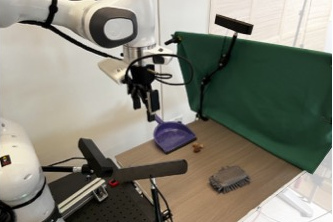
\includegraphics[height=1.10cm]{figures/generated/literature_review/openvla_scene.jpg}};
  \node[laSource] at (1.60,4.56) {OpenVLA};
  \node[laRoute] at (4.20,4.98) {VLA};
  \node[laSlot,minimum width=2.35cm] at (\cIn,4.98) {观测＋任务};
  % the arrow crosses the empty prediction column on purpose
  \draw[laArrow] (8.32,4.98) -- (12.28,4.98);
  \node[laSource,fill=white,inner xsep=3pt] at (\cPred,4.98) {不经预测};
  \node[laSlot,minimum width=2.55cm] at (\cOut,4.98) {动作};

  \draw[black!20,line width=0.4pt] (\rowSep,4.16) -- (\rowSepEnd,4.16);

  % ---------- row 2: prediction-assisted operation ----------
  \node at (1.60,3.40)
    {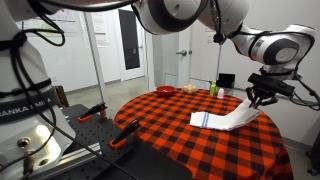
\includegraphics[height=1.10cm]{figures/generated/literature_review/point_observation_v1.jpg}};
  \node[laSource] at (1.60,2.66) {PointWorld};
  \node[laRoute] at (4.20,3.08) {预测辅助\\操作};
  \node[laSlot,minimum width=2.35cm] at (\cIn,3.08) {状态＋\\候选动作};
  \draw[laArrow] (8.32,3.08) -- (9.30,3.08);
  \node[laPred,minimum width=1.90cm] at (\cPred,3.08) {预测后果};
  \draw[laArrow] (11.34,3.08) -- (12.28,3.08);
  \node[laSlot,minimum width=2.55cm] at (\cOut,3.08) {动作选择};

  \draw[black!20,line width=0.4pt] (\rowSep,2.26) -- (\rowSepEnd,2.26);

  % ---------- row 3: world action model ----------
  \node at (1.60,1.50)
    {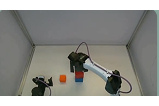
\includegraphics[height=1.10cm]{figures/generated/literature_review/dreamzero_scene.jpg}};
  \node[laSource] at (1.60,0.76) {DreamZero};
  \node[laRoute] at (4.20,1.18) {WAM};
  \node[laSlot,minimum width=2.35cm] at (\cIn,1.18) {观测＋任务};
  \draw[laArrow] (8.32,1.18) -- (9.30,1.18);
  % one slot spanning prediction and output: the two are generated together
  \node[laPred,minimum width=5.85cm] at ({(9.30+15.15)/2},1.18)
    {未来视频＋动作\quad{\fontsize{8.5pt}{10.5pt}\selectfont（联合生成）}};
\end{tikzpicture}
\endgroup
}
\caption{具身操作的典型建模范式}
\label{fig:literature-action-paradigms}
\end{figure}

在预测辅助操作中，环境预测可以通过动作比较和策略学习进入操作过程。潜在动力学模型利用想象轨迹训练行为，DINO-WM 通过预测特征中的目标误差优化动作，PointWorld 则将三维响应预测用于模型预测控制\cite{ref02,ref03,ref06}。在这些使用方式中，预测需要保留会影响目标达成和动作可执行性的场景差异；新的真实观测又为状态修正及后续动作提供依据。因此，预测误差和任务收益之间的联系，取决于状态表达、动作选择方式及反馈条件，几何或视觉预测指标的改善需要通过实际操作进一步检验。

世界动作模型进一步将未来世界状态和动作共同建模。近期的 DreamZero 以预训练视频扩散模型为基础，联合建模未来视频和机器人动作，探索视觉演化先验对跨任务及跨环境操作的支持\cite{dreamzero2026}。这一形式使环境变化和动作生成在同一过程中建立联系。对本课题而言，给定动作是场景演化的条件；联合生成未来动作的能力则提供了另一种预测使用方式，二者的输入输出角色和使用目标需要明确区分。

真实示范和任务基准为操作研究提供了不同层次的评价条件。BridgeData V2 与 DROID 分别汇集真实机器人操作数据\cite{bridgedata2023,droid2024}；RLBench 提供多任务机器人学习环境，LIBERO 和 CALVIN 分别侧重任务间知识迁移及语言条件下的长程操作\cite{rlbench2020,libero2023,calvin2022}。数据采集方式、动作接口和任务成功条件的差异会影响训练及评价结果的可比性。

仿真基准可进一步支持受控的操作比较。RoboCasa 面向日常家庭操作场景，RoboTwin 提供双臂操作任务，SIMPLER 则研究在仿真中评价真实机器人操作策略\cite{robocasa2024,robotwin2025,simpler2025}。这些资源提供任务及环境设计的参考；仿真结果能否迁移到实际设备，还需结合观测、动作接口及场景差异进行验证。

这些方式可以在操作系统中相互结合。代表性操作可从动作后果预测、动作选择及反馈执行三个层面，检验连续动态状态的使用价值，为本课题认识状态构建同交互预测的有效联系提供依据。

\Needspace{110pt}
\subsection{已有工作积累及研究基础}

\subsubsection{连续时间重建的前期探索}

前期工作 CoFuse4D 暂定题目为 \textit{CoFuse4D: Dense Correspondence Fusion for Dynamic Gaussian Splatting}，围绕三维高斯场景中的带噪稠密对应融合、有限复杂度的运动支撑及时间高斯过程开展探索，关注运动和几何质量，以及动态重建和新视角合成效果。这些经验为第一项研究中的多时刻证据利用和连续运动表达提供了基础，也为后续空间组织研究提供运动状态的实现参考。后续将进一步围绕观测约束、表示自由度及其对几何累积的作用开展研究。该工作尚未发表，计划投稿至 CVPR 2027。

\subsubsection{动作条件状态学习的前期探索}

前期工作 PS-VLA 暂定题目为 \textit{PS-VLA: Learning Action-Conditioned Predictive States for Robotic Manipulation}，在 BridgeVLA 操作框架\cite{ref12}基础上，探索持续潜在状态、动作条件转移及观测更新。在新观测进入状态更新前，根据历史状态和动作预测相关特征，再利用观测修正状态。这些探索为第四项研究提供了状态学习和操作模型的实现经验。后续将进一步研究前三项场景信息进入交互状态的方式，以及它们对动作后果预测的实际作用。该工作同样尚未发表，计划投稿至 CVPR 2027。


\clearpage
\npuBlock*{学位论文研究内容}{学位论文的研究目标、研究内容及拟解决的关键性问题（可续页）}
% !TeX root = ../main.tex
\subsection{研究目标}

本课题面向三维动态场景，研究连续动态世界模型的构建方法。所建模型由可持续更新的连续场景状态和基于状态的动作条件演化关系组成：利用可用时序视觉观测构建几何、外观及运动状态，依据新增证据调整空间组织和有效结构，再以当前状态及给定动作推演后续变化。研究围绕物体运动、相互遮挡及局部结构变化展开，以代表性具身操作检验所建模型的预测及使用价值。

总体目标是建立由离散观测构建连续状态、组织空间结构、适应局部变化并学习动作条件演化的方法，形成具有明确状态接口的连续动态世界模型研究原型。预期所得状态时间上连续可查询、空间归属稳定，并能在真实局部结构改变后保留有效历史。通过代表性动态场景和选定操作任务，检验各类构建方法对状态恢复及动作后果预测的作用，阐明其成立条件和适用范围。

本课题中的“连续”以场景运动的连续时间表达为基础，使不同采样时刻的观测联系到同一状态过程，并支持状态随新增观测持续更新。结构保持时延续可信联系，发生切割、撕裂等事件时局部调整连接关系和表面集合，保留未受影响区域的有效历史。时空一致性作为状态构建及演化预测的质量要求；研究以可用观测支持的内容为基础，观测不足处保留信息缺失，预测初始状态仅依据当时已经获得的观测和动作历史构建。具体目标如下。

（1）\textbf{构建连续可查询的场景状态。}以离散观测约束场景的连续运动过程，使不同采样时刻的信息在统一的时间表征中建立联系，支持非采样时刻查询和多时刻几何信息累积，为世界模型建立连续时间状态基础。

（2）\textbf{构建空间组织稳定的连续场景状态。}在连续时间状态基础上，以对象或部件组织空间成分，使已有观测和首次显露的表面获得一致的空间归属，支持空间单元内的几何信息累积及运动状态读取，为后续演化提供可组织的空间结构。

（3）\textbf{形成适应拓扑变化的动态表面更新方法。}面向切割、撕裂引起的连接关系改变和物理边界新生，调整失效的结构联系，在延续未变化区域可信信息的基础上更新局部表面，使场景状态能够适应真实结构变化。

（4）\textbf{建立连续状态驱动的动作条件演化模型。}利用连续运动、空间归属及当前有效结构学习给定动作下的场景演化，研究从动态初始状态预测后续变化的方法，检验所得世界模型在预测准确性、一致性及操作中动作选择方面的作用。

\Needspace{110pt}
\subsection{研究内容}

四项研究共同服务于连续动态世界模型的构建。第一项由离散观测构建连续时间状态；第二项利用连续运动建立对象或部件的稳定空间组织；第三项依据观测更新真实结构改变后的有效联系和局部表面；第四项基于所得状态建立动作条件演化关系。前三项形成模型的状态基础，第四项使模型能够推演动作后果。各项分别检验其构建机制，并通过可读取的场景状态逐步衔接。

\subsubsection{连续时间场景状态构建}

动态场景的观测通常按离散时刻采集。以逐时刻状态或相邻帧变换组织运动时，采样时刻之间的演化需要额外的插值或一致性约束，长时间跨度内的几何信息累积也容易受到局部估计误差影响。连续时间建模通过共享的时间函数描述运动过程，使离散观测能够在同一表征中建立联系，为非采样时刻的状态查询和跨时刻几何信息累积提供统一的表达基础。

近年来，动态高斯场景中的连续运动表征逐步发展，已有研究通过时间变形函数、样条轨迹或连续动力学描述场景演化，为连续建模提供了基础\cite{gs4d2024,retimegs2026,particlegs2026}。在复杂动态场景中，连续模型仍面临运动表达能力和观测约束如何匹配的问题：过强的时间约束可能抹去真实的局部变化，过高的运动自由度可能吸收观测噪声，而不同时刻的观测质量和运动变化又会影响几何信息的融合。因此，需要进一步研究连续运动的表达能力同有效观测约束之间的匹配关系。

本项拟研究离散观测约束下的连续时间场景状态构建方法，探索运动表达能力同观测条件相匹配的建模方式，建立多时刻证据对连续运动的有效约束，使几何信息能够沿一致的运动过程累积，形成可查询几何、外观及运动信息的连续状态，作为后续空间组织、结构更新和演化建模的基础。

\subsubsection{连续运动引导的结构化空间表征}

连续时间表征能够描述场景演化，但仍需确定空间成分的归属及信息共享范围。空间邻近或短时运动相似未必意味着同一对象，同一对象内部也可能存在不同部件运动。物体旋转、部件运动或遮挡解除会使已有表面首次进入观测，需要将新观测纳入所属空间单元，完善对已有结构的表征。

已有研究通过运动支撑图、共享运动基和实例信息联系时间运动和空间组织\cite{ref05,shapeofmotion2025,consistentinstance2026}。运动分组同对象身份的关系、观测不充分时的归属可靠性及空间约束对连续状态恢复的作用仍值得研究。本项主要关注物理连接保持时的空间组织，表面首次显露不等同于物理边界新生。

本项拟在连续时间场景状态基础上，研究连续运动证据引导的结构化空间表征方法。结合几何、外观和可见性信息，探索空间归属的建立及延续方式，以对象或部件组织共享运动和局部几何约束，将首次显露的已有表面纳入一致的空间状态，并减少不同单元之间的错误信息传递。预期形成空间归属稳定、能够持续累积几何信息并分别读取对象或部件状态的表示，为世界模型提供有效的空间组织。

\subsubsection{拓扑变化下的动态表面更新}

在连续运动和空间组织基础上，切割、撕裂还会改变物体连接关系，并使内部材料成为新的物体边界。变化前的邻接或共享运动约束可能失效，沿用旧联系容易错误绑定已分离区域，整体放弃历史又会损失稳定区域的有效信息，因此需要适应真实拓扑变化的动态表面表征。

已有方法通过高斯逐帧更新、局部解绑或表面重建适应动态几何变化，为本项提供了直接参考\cite{gaustar2025,atgs2025}。面向真实切割、撕裂，需要进一步研究跨时刻对应、邻接关系及共享运动约束在变化区域的适用范围，并依据物理边界变化更新表面表示。此前未被观测不足以说明表面在物理上新生，区分可见性变化和真实结构变化是避免错误更新的重要条件。

本项拟在结构化场景状态基础上，研究局部变化证据约束的动态表面更新方法。探索历史联系的保留和调整条件，使稳定区域延续可信的运动及几何历史，变化区域解除失效连接，并为真实新生表面建立符合其形成过程的表示。通过在结构事件处局部更新表面集合和连接关系，使连续场景状态能够延续到变化后的有效结构，为后续演化建模提供依据。

\subsubsection{连续状态驱动的动作条件演化建模}

现有面向交互的世界模型围绕图像特征预测、三维场景生成和给定动作下的三维点运动预测等方向开展研究，并将所得预测用于动作规划或策略学习\cite{ref03,gwm2025,ref06}。不同方法分别侧重预训练视觉特征的利用、未来场景的生成或三维交互响应，历史信息和空间先验也已被部分研究引入，为基于场景状态的交互建模提供了基础。

在场景已处于运动、局部观测缺失或物理连接改变的条件下，当前几何相近的状态仍可能具有不同的动作响应。连续运动历史有助于确定动态初始状态，对象和部件归属支持局部交互信息的组织，当前有效连接关系影响局部区域之间的响应关联。已有研究对这些信息的使用方式和支持条件各有侧重，仍需研究如何将持续更新的时空结构状态转化为动作条件预测的有效约束。

本项拟基于前三项形成的连续场景状态，研究动作条件演化关系的构建方法。以截至预测时刻已经恢复的运动和结构为起点，依据对象或部件组织局部交互信息，利用当前有效的连接和边界约束响应预测，学习给定动作下的后续几何和运动变化，使所建世界模型能够从状态恢复进一步推演动作后果。结合新增观测更新状态，并在代表性具身操作任务中检验预测及动作选择的实际效果，明确状态构建的改进能够转化为预测收益的条件。预测初始状态仅依据当时已经获得的观测和动作历史构建。

\Needspace{110pt}
\subsection{拟解决的关键科学问题}

本课题关注的总体问题是：有限离散观测如何约束连续场景状态的可靠构建及其动作条件演化？围绕连续状态构建、稳定空间组织、结构变化适应和动作后果预测，具体提炼以下四个相互关联的科学问题，分别对应四项模型构建内容。

\subsubsection{离散观测对连续场景运动的有效约束}

离散观测在什么条件下能够有效约束连续场景运动？有限采样只能提供部分时刻的状态证据，连续时间形式本身不能保证帧间演化的准确性。需要研究采样条件、观测可靠性及运动复杂程度如何共同影响连续运动恢复，阐明运动表达自由度同有效观测约束之间的匹配关系，以及所得运动描述对多时刻几何信息累积的影响。该问题对应第一项研究内容，重点认识由离散证据构建可靠连续状态的条件。

\subsubsection{连续运动支持稳定空间组织的条件}

连续时间运动证据如何支持稳定的空间组织？局部运动相似和空间邻近不足以单独确定对象或部件的归属，已有表面首次显露时也缺少此前的直接观测对应。需要研究运动过程中的几何、外观和可见性证据如何互补，阐明可靠空间归属的建立条件，以及由此形成的共享约束如何作用于连续运动和几何恢复。该问题对应第二项研究内容，重点认识连续运动支持空间归属形成及延续的条件。

\subsubsection{拓扑变化下结构约束的有效范围}

真实拓扑变化发生时，哪些历史结构联系能够延续，哪些需要调整？表面首次显露和物理边界新生都可能缺少此前的直接观测对应，仅凭对应缺失不足以确定结构已经改变。需要研究局部几何及运动证据如何约束连接失效的判断，阐明结构变化对邻接联系、共享运动约束及表面历史的不同要求，使可信约束在稳定区域延续、在变化区域适应性调整。该问题对应第三项研究内容，重点认识真实结构变化下历史约束的有效范围及其对表面更新的作用。

\subsubsection{连续场景状态对动作后果的有效约束}

连续场景状态在什么条件下能够有效约束动作后果？相近的瞬时几何可能对应不同的运动历史和连接状态，连续可查询或几何精度提高本身不能保证后续响应预测准确。需要研究连续运动、对象或部件组织及有效结构联系如何共同影响动作条件演化，阐明这些信息在观测不充分或局部结构改变时的作用范围，以及状态估计误差如何影响预测可靠性。该问题对应第四项研究内容，重点认识世界模型中连续状态同动作条件演化之间的有效联系及适用条件。


\clearpage
\npuBlock*{学位论文研究计划及预期目标}{1.拟采取的主要理论、研究方法、技术路线和实施方案（可续页）}
% !TeX root = ../main.tex
% 第三部分仅保留学校模板的三个栏目、空研究计划表和末页备注栏。
% 第一个栏目及填写要求在主文件中给出，以下留白用于后续编写。
\vspace*{45mm}

\npuTemplateHeading{2.研究计划可行性，研究条件落实情况，可能存在的问题及解决办法（可续页）}
\vspace*{45mm}

\npuTemplateHeading{3.研究计划及预期成果}
\npuSchedule{%
  \rule{0pt}{12mm} & \\\hline
  \rule{0pt}{12mm} & \\\hline
  \rule{0pt}{12mm} & \\\hline
  \rule{0pt}{12mm} & \\
}

\npuFinish

\clearpage
% !TeX root = ../main.tex
% 文献列表独立置于报告末尾，使用第四部分标题；按正文首次引用顺序编号。
\bibliographystyle{npu-gbt7714-numerical}
\bibliography{references}

\end{document}
